\chapter[Apéndice: Manual de usuario]{
  \label{chp:usermanual}
  Manual de usuario
}

Neste apéndice apórtase un manual de referencia para os usuarios da web.

\begin{figure}[h]
	\centering
	\fbox{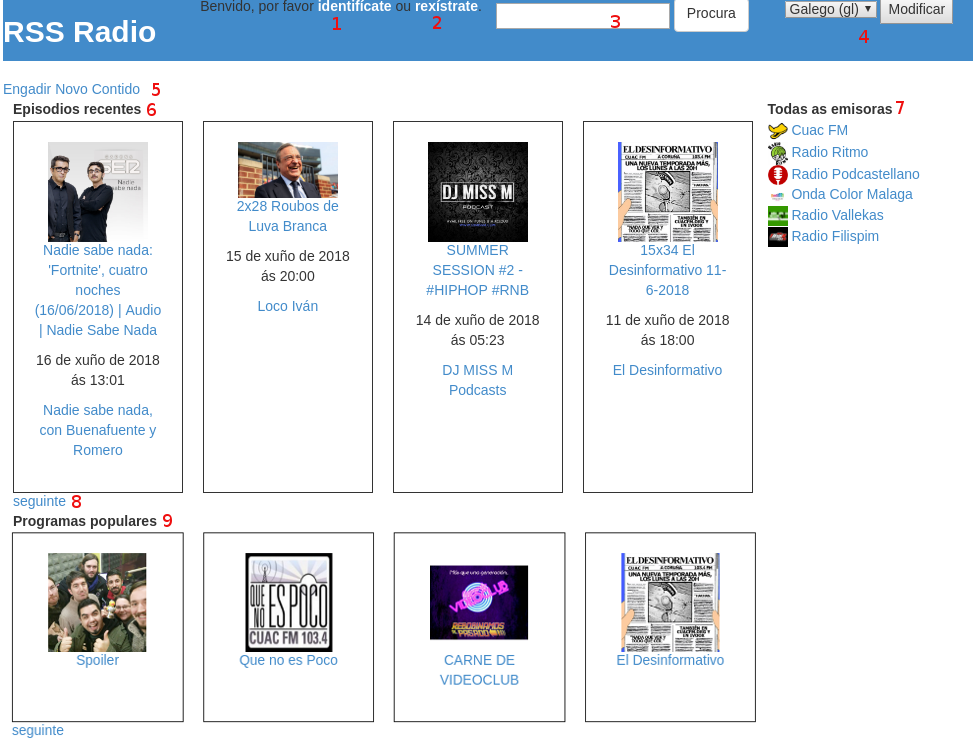
\includegraphics[scale=0.43,keepaspectratio=true]{./images/usermanual/um-index-anon.png}}
	\caption{Portada da web para usuario anónimo}
	\label{fig:um-index-anon}
\end{figure}

Na figura \ref{fig:um-index-anon} amósase o aspecto da portada da web para un usuario anónimo con números identificando as distintas áreas:

\begin{itemize}
	\item \textbf{1:} Enlace á páxina de login.
	\item \textbf{2:} Enlace á páxina de rexistro.
	\item \textbf{3:} Caixa de procura por texto.
	\item \textbf{4:} Selector de idioma.
	\item \textbf{5:} Enlace ao menú de creación de novo programa e emisora. Require identificación.
	\item \textbf{6:} Sección de episodios recentes. Amósanse os 4 últimos episodios engadidos ao sistema independentemente do seu programa. Para ver os 4 seguintes, pódese premer o botón marcado co \textbf{8}.
	\item \textbf{7:} Lista de emisoras presentes no sistema.
	\item \textbf{8:} Botón para cargar a seguinte páxina.
	\item \textbf{9:} Sección de programas ordenados por popularidade. Amósanse os 4 primeiros tamén con opción de cargar a seguinte páxina.  
\end{itemize}

\section{Usuarios}

\subsection{Crear}
Para crear un novo usuario, prémese un botón \textbf{2} da figura \ref{fig:um-index-anon}. Cargarase a páxina de rexistro de usuario. Basta con cubrir os campos como se amosa no exemplo da figura \ref{fig:um-signup}. Se non hai ningún erro, o usuario quedará autenticado e será redirixido á súa páxina de detalles (figura \ref{fig:um-userd1})



\subsection{Editar}
Para acceder ao menú de edición de usuario, prémese o botón de edición marcado co \textbf{10} na figura \ref{fig:um-userd1}. O menú de edición pódese ver na figura \ref{fig:um-edituser}. Nótese que o nome de usuario non é editable e que o cambio de password é un formulario aparte.

Se a edición se completa de forma correcta, vólvese á vista de detalles de usuario.

\begin{figure}[H]
	\centering
	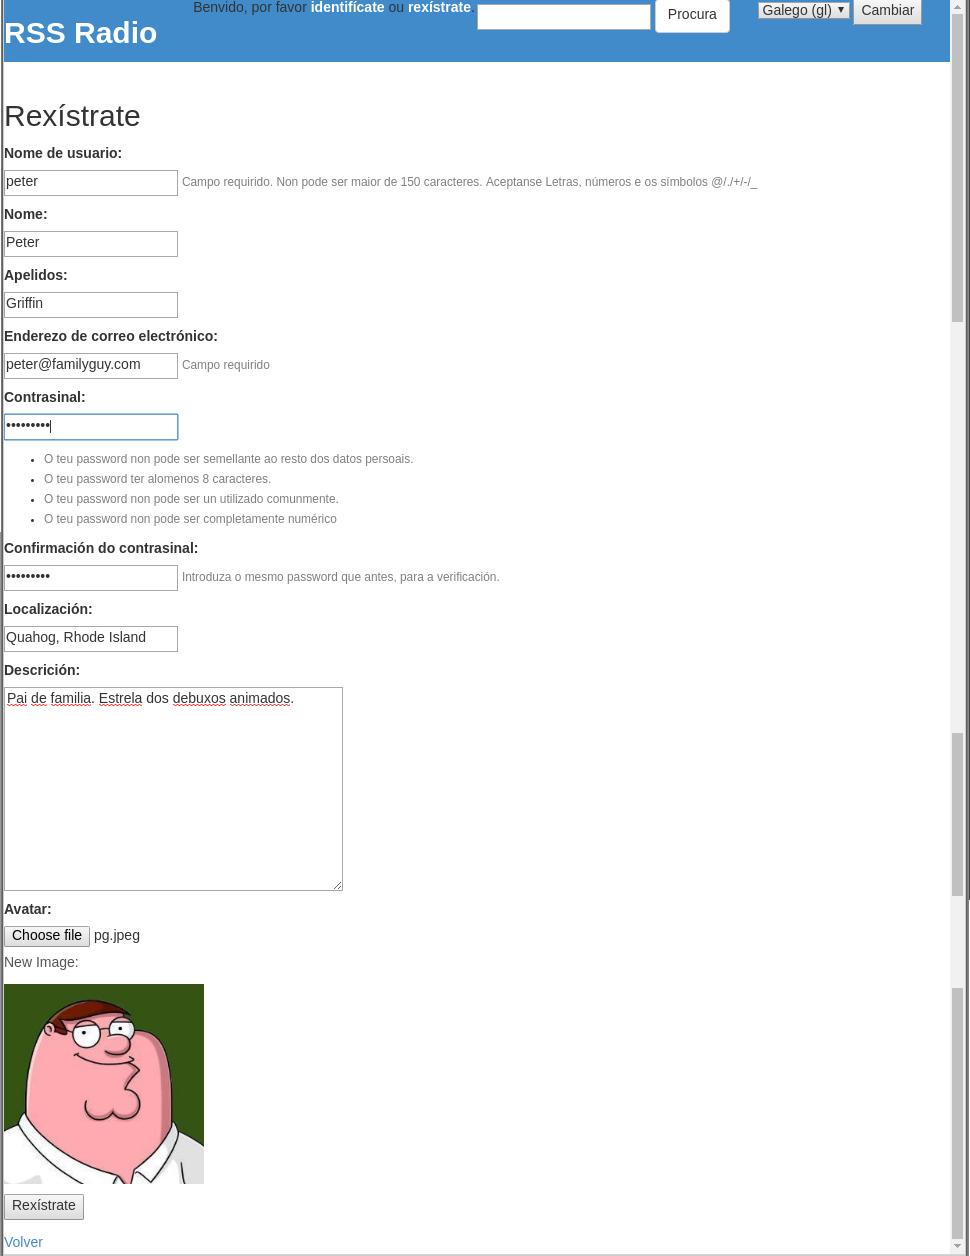
\includegraphics[scale=0.43,keepaspectratio=true]{./images/usermanual/um-signup.png}
	\caption{Rexistro de usuario.}
	\label{fig:um-signup}
\end{figure}


\begin{figure}[H]
	\centering
	\fbox{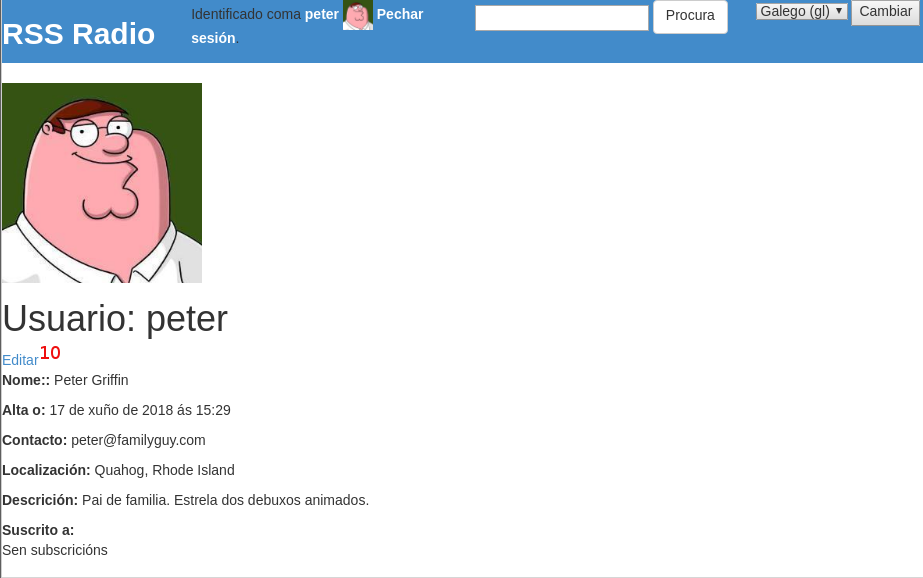
\includegraphics[scale=0.45,keepaspectratio=true]{./images/usermanual/um-userd1.png}}
	\caption{Detalles de usuario. Información do perfil.}
	\label{fig:um-userd1}
\end{figure}


\begin{figure}[H]
	\centering
	\fbox{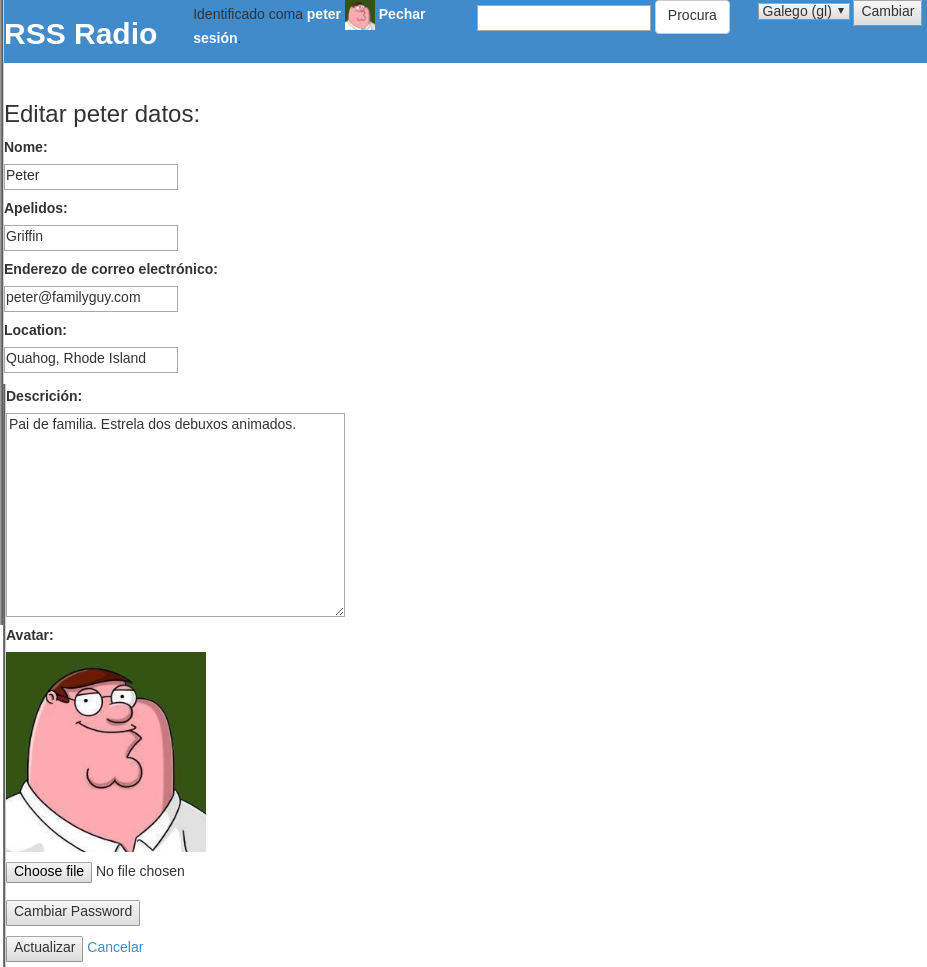
\includegraphics[scale=0.45,keepaspectratio=true]{./images/usermanual/um-edituser.png}}
	\caption{Editar usuario.}
	\label{fig:um-edituser}
\end{figure}


\section{Accións de ouvinte}

\subsection{Escoitar e seguir unha emisora}

Para realizar accións sobre unha emisora cómpre ir á súa páxina de detalles. As emisoras poden ser \say{seguidas} polos usuarios como forma de engadila a \say{favoritas}. A continuación explícanse os elementos da páxina de detalles de emisora marcados na figura \ref{fig:um-stationd1}.

\begin{itemize}
	\item \textbf{11:} Botón de seguimento.
	\item \textbf{12:} Reprodutor de emisión en directo.
	\item \textbf{13:} Lista dos últimos episodios publicados ordenada por data.
	\item \textbf{14:} Lista de programas emitidos pola emisora.
	\item \textbf{15:} Usuarios seguidores  da emisora.
\end{itemize}


\subsection{Subscribirse a un programa}

Para subscribirse ou cancelar unha subscrición previa, o usuario debe ir á páxina de detalles do programa en cuestión. A continuación explícanse os elementos da páxina de detalles de programa marcados na figura \ref{fig:um-programd1}.

\begin{itemize}
	\item \textbf{16:} Botón de subscrición.
	\item \textbf{17:} Enlace á páxina de resultados de busca polo tag \say{comedy}.
	\item \textbf{18:} Lista dos últimos episodios ordenada por data de publicación dos audios.
	\item \textbf{19:} Lista de emisoras nas que se emite o programa.
	\item \textbf{20:} Usuarios subscritos ao programa.
\end{itemize}

\subsection{Accións sobre os episodios}

Accedendo á vista de detalles de episodio pódese escoitar mediante streaming ou descargar o ficheiro de audio. Os episodios poden votarse e comentarse.  A continuación explícanse os elementos da páxina de detalles de episodio marcados na figura \ref{fig:um-episoded1}.

\begin{itemize}
	\item \textbf{21:} Botóns de voto positivo ou negativo. O usuario sempre pode desfacer ou cambiar o seu voto.
	\item \textbf{22:} Reprodutor do ficheiro de audio do episodio.
	\item \textbf{23:} Enlace á páxina de resultados de busca por tag (Neste exemplo, o episodio non ten tags de seu.)
	\item \textbf{24:} Sección de comentarios do episodio.
\end{itemize}

\begin{figure}[H]
	\centering
	\fbox{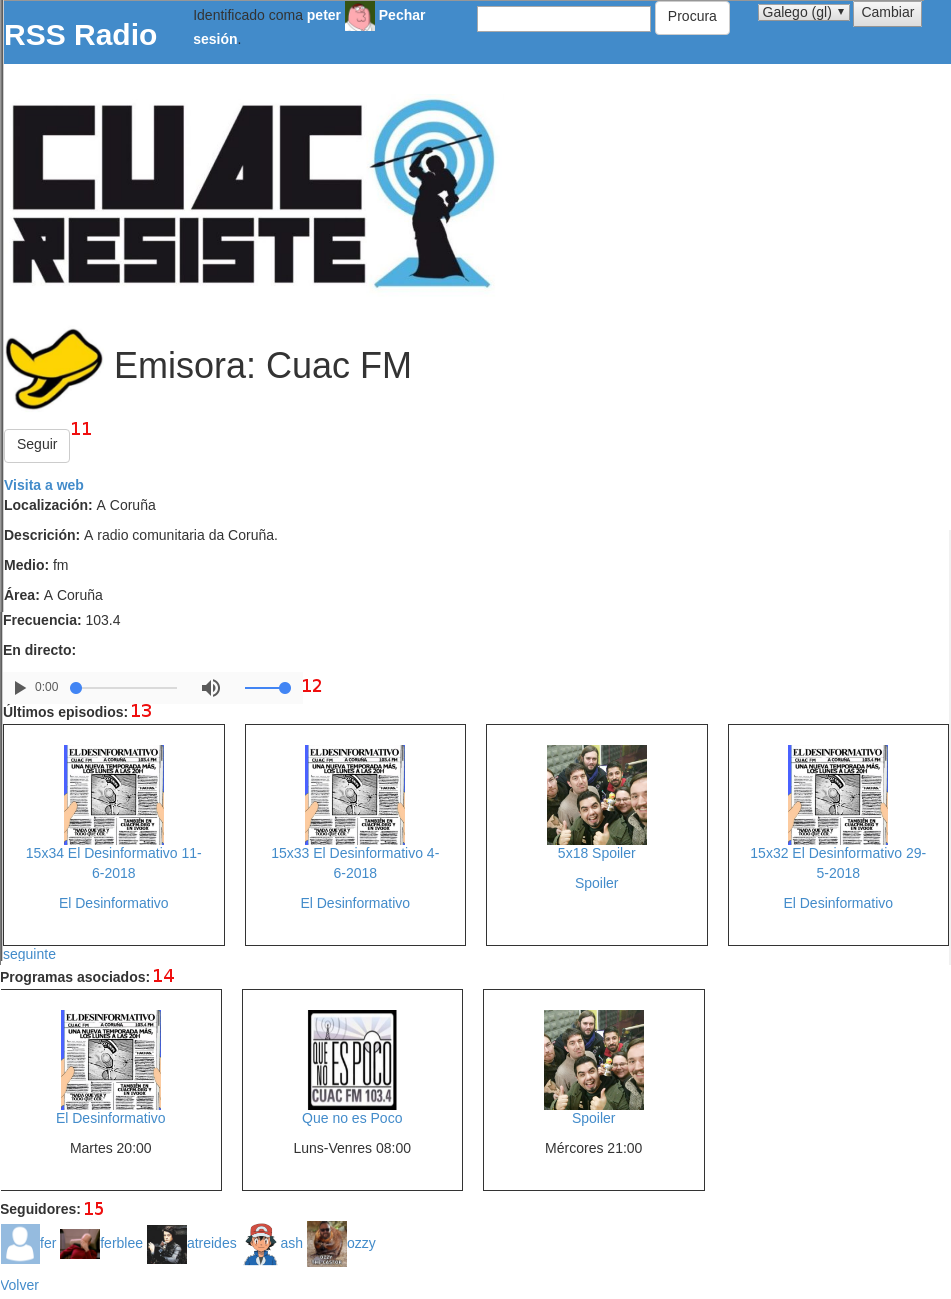
\includegraphics[scale=0.45,keepaspectratio=true]{./images/usermanual/um-stationd1.png}}
	\caption{Detalles de emisora.}
	\label{fig:um-stationd1}
\end{figure}

\begin{figure}[H]
	\centering
	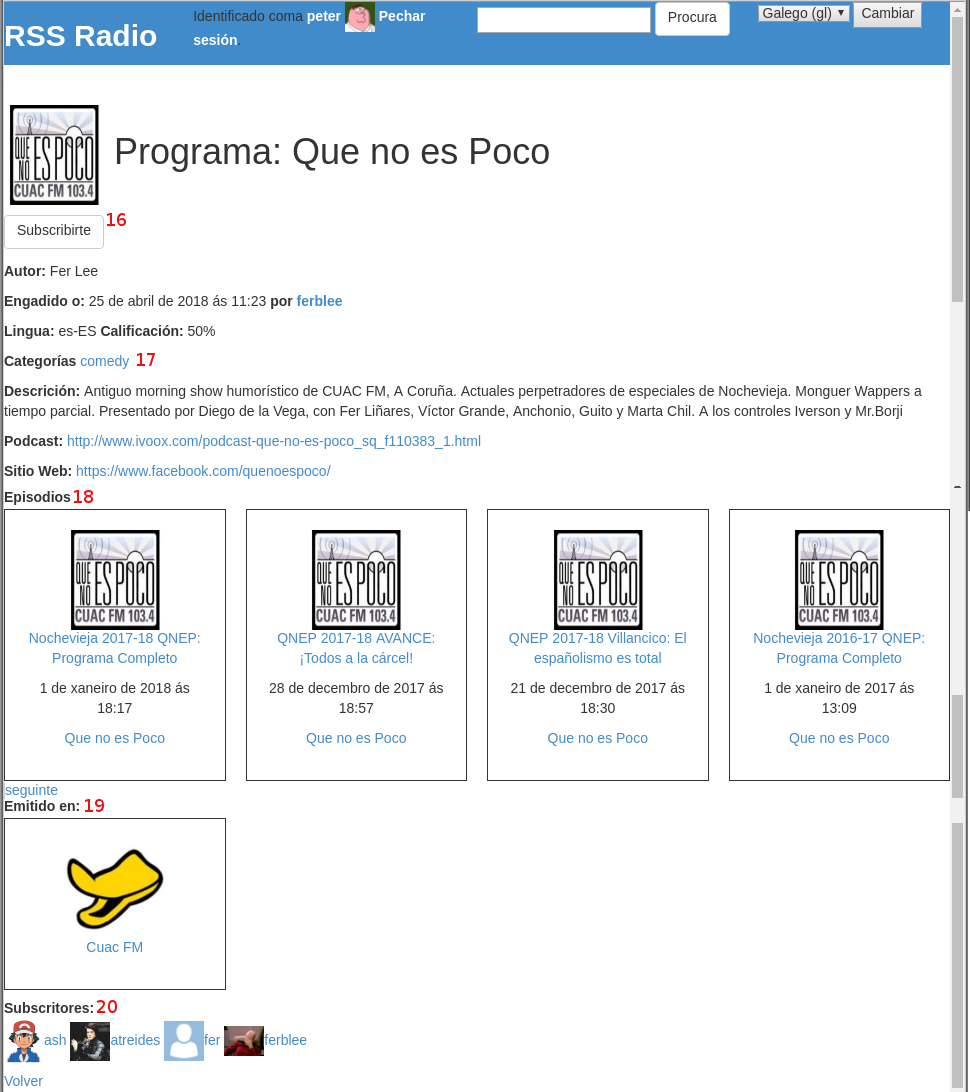
\includegraphics[scale=0.45,keepaspectratio=true]{./images/usermanual/um-programd1.png}
	\caption{Detalles de programa.}
	\label{fig:um-programd1}
\end{figure}


\begin{figure}[H]
	\centering
	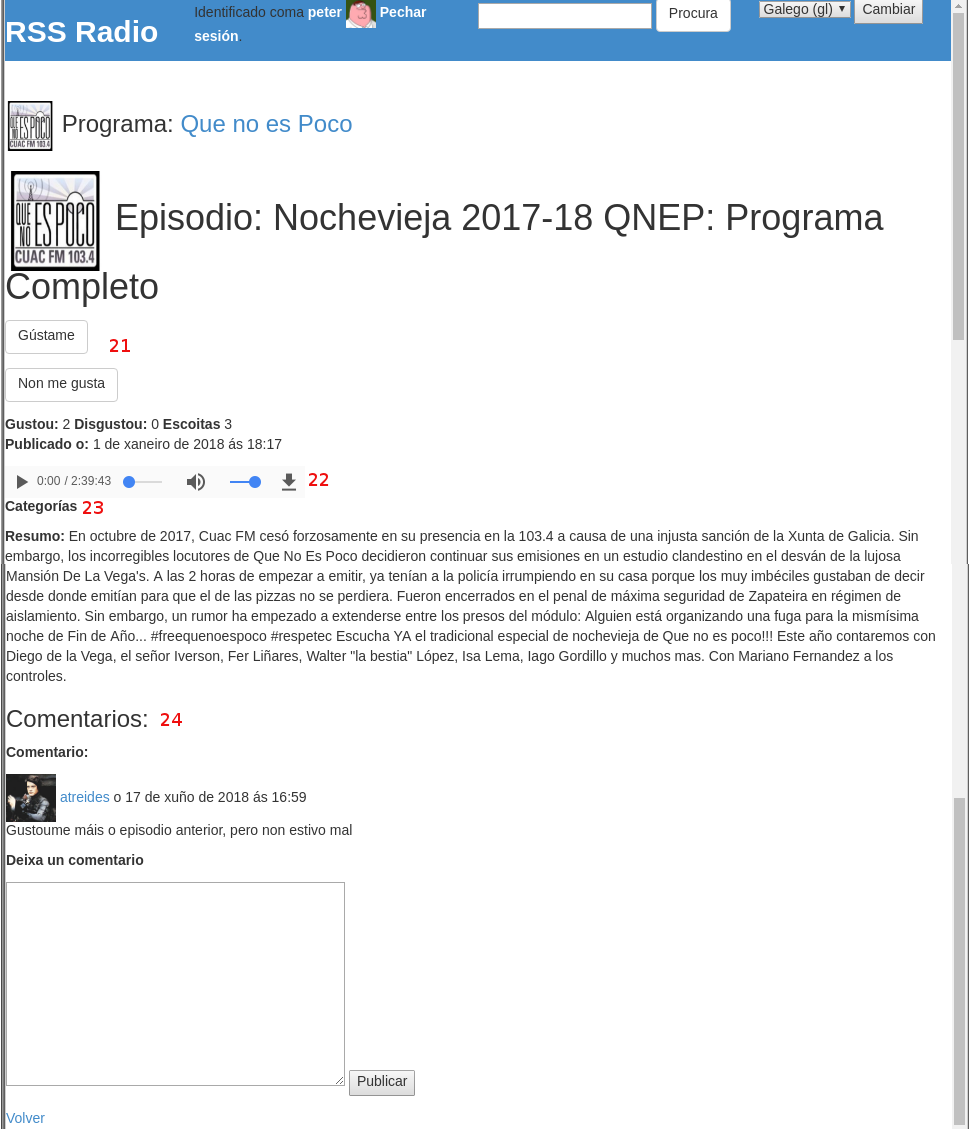
\includegraphics[scale=0.45,keepaspectratio=true]{./images/usermanual/um-episoded1.png}
	\caption{Detalles de episodio.}
	\label{fig:um-episoded1}
\end{figure}

\subsection{Contidos favoritos}

Nos exemplos anteriores, o usuario seguiu unha emisora e subscribiuse a un programa. Este contido está agora dispoñible de xeito máis fácil desde a portada e máis desde o seu perfil como se pode ver nas figuras \ref{fig:um-index-auth} e \ref{fig:um-userd2}.

\begin{figure}[H]
	\centering
	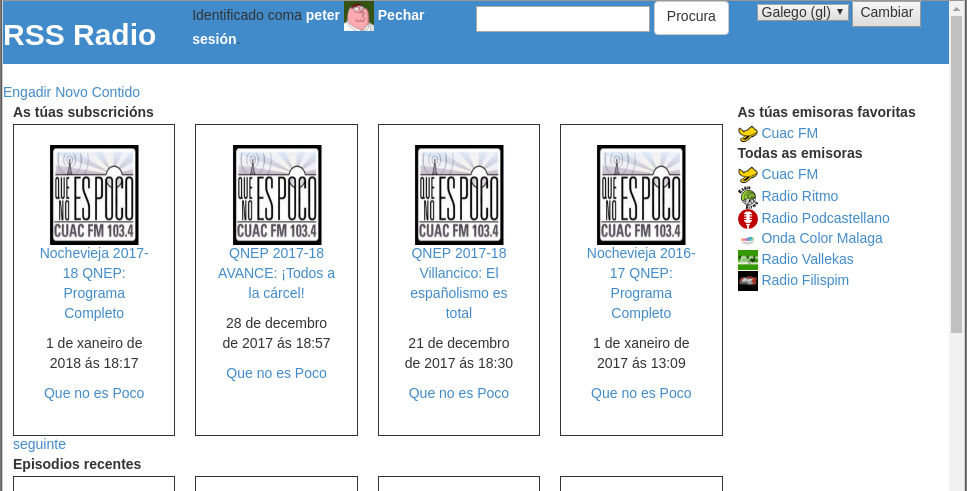
\includegraphics[scale=0.45,keepaspectratio=true]{./images/usermanual/um-index-auth.png}
	\caption{Contidos favoritos na portada.}
	\label{fig:um-index-auth}
\end{figure}


\begin{figure}[H]
	\centering
	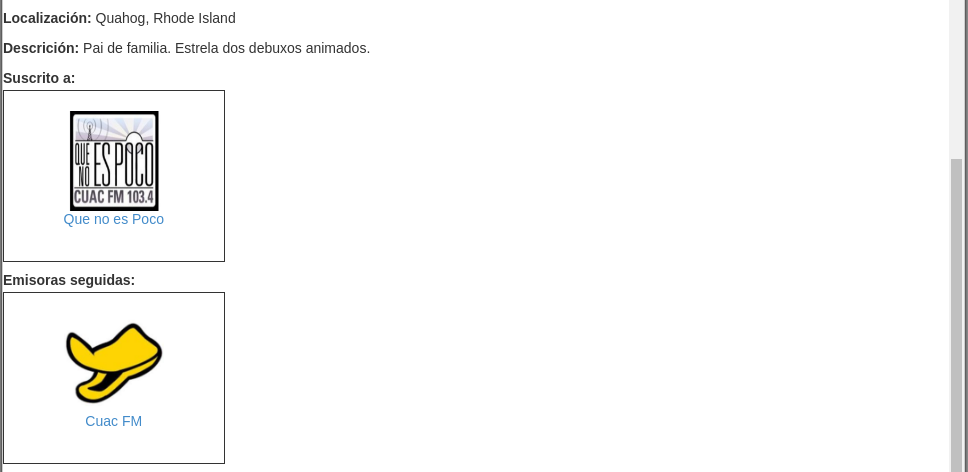
\includegraphics[scale=0.45,keepaspectratio=true]{./images/usermanual/um-userd2.png}
	\caption{Contidos favoritos na vista de perfil de usuario.}
	\label{fig:um-userd2}
\end{figure}


\section{Procura de contidos}

O sistema proporciona 2 formas de procura de contidos: Por texto, mediante a caixa marcada co \textbf{3} na figura \ref{fig:um-index-anon} , ou por tag, premendo nos enlaces correspondentes (Ver número \textbf{17} na figura \ref{fig:um-programd1}). Ambas levan á páxina de resultados de procura, onde se amosarán os episodios, programas, emisoras e usuarios que cumpran os criterios da busca.

Na figura \ref{fig:um-search} móstrase un exemplo de procura pola palabra \say{radio}.

\begin{figure}[H]
	\centering
	\fbox{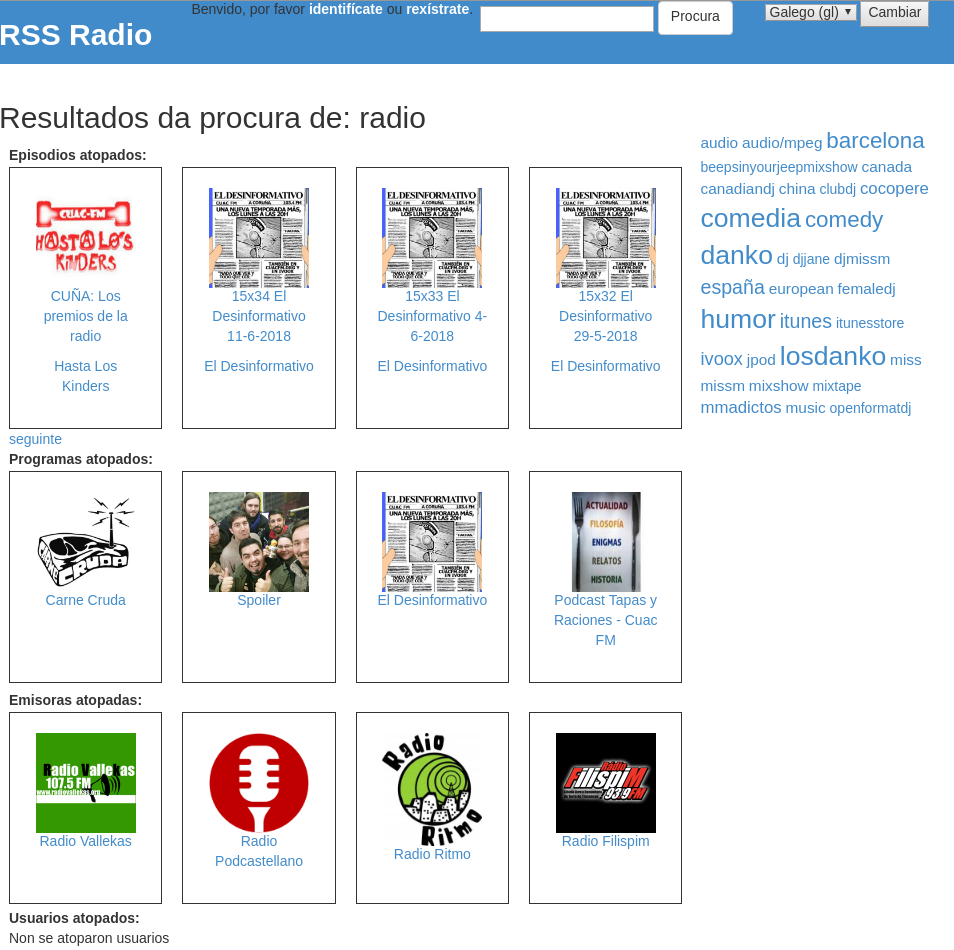
\includegraphics[scale=0.45,keepaspectratio=true]{./images/usermanual/um-search.png}}
	\caption{Páxina de resultados de procura. Exemplo de busca pola palabra radio.}
	\label{fig:um-search}
\end{figure}


\section{Accións de produtor de contidos}

\subsection{Crear unha emisora}

Para engadir unha emisora, o usuario ten que ir á vista de \say{engadir contido}, mediante o enlace marcado co \textbf{5} na figura 	\ref{fig:um-index-anon}. Unha vez alí, cóbrense os campos do formulario como se ve na figura \ref{fig:um-add-station}

Se os datos introducidos son correctos, rediríxese ao usuario á páxina de detalles da nova emisora (figura \ref{fig:um-stationd2}). O usuario creador da emisora ten permisos de \say{propietario} sobre a citada emisora.


\subsection{Xestionar unha emisora}

Se o usuario é propietario ou xestor dunha emisora, poderá ver o botón marcado coma \textbf{25} na figura \ref{fig:um-stationd2}. Este levaralle ao panel de xestión da emisora, no que se poden realizar as seguintes operacións:

\subsubsection{Editar perfil}

Vista amosada na figura \ref{fig:um-edstation1}. Desde ahí pódense editar os datos do perfil da emisora.


\subsubsection{Xestionar emisión}
\label{xe}

Vista amosada na figura \ref{fig:um-edstation2}. Desde aí pódense engadir programas á emisión e retiralos da mesma.

\begin{itemize}
	\item \textbf{26:} Selector de programa. Úsase para seleccionar o programa que se queira engadir á emisión.
	\item \textbf{27:} Caixa de texto para especificar o horario de emisión do programa a engadir.
	\item \textbf{28:} Área de programas xa emitidos. Ás filas seleccionadas aplicaráselles á acción definida en \textbf{29}.
	\item \textbf{29:} Botóns de acción. Determinan se os programas seleccionados son para borrar ou para actualizar os seus datos de emisión.
\end{itemize}

\begin{figure}[H]
	\centering
	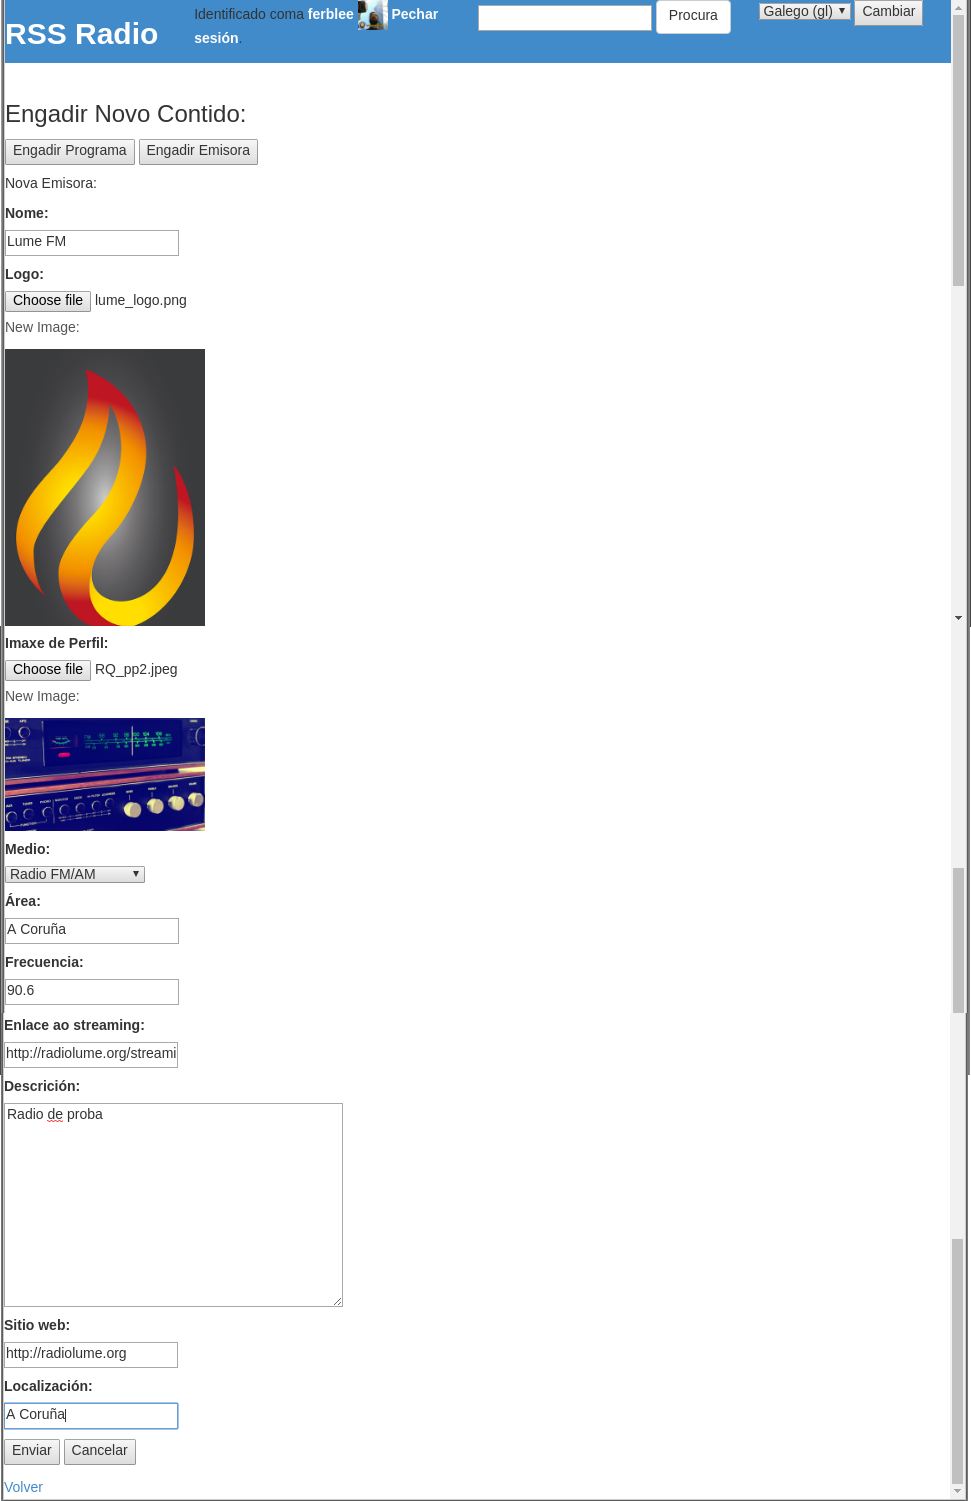
\includegraphics[scale=0.4,keepaspectratio=true]{./images/usermanual/um-add-station.png}
	\caption{Engadir emisora.}
	\label{fig:um-add-station}
\end{figure}

\break

\begin{figure}[H]
	\centering
	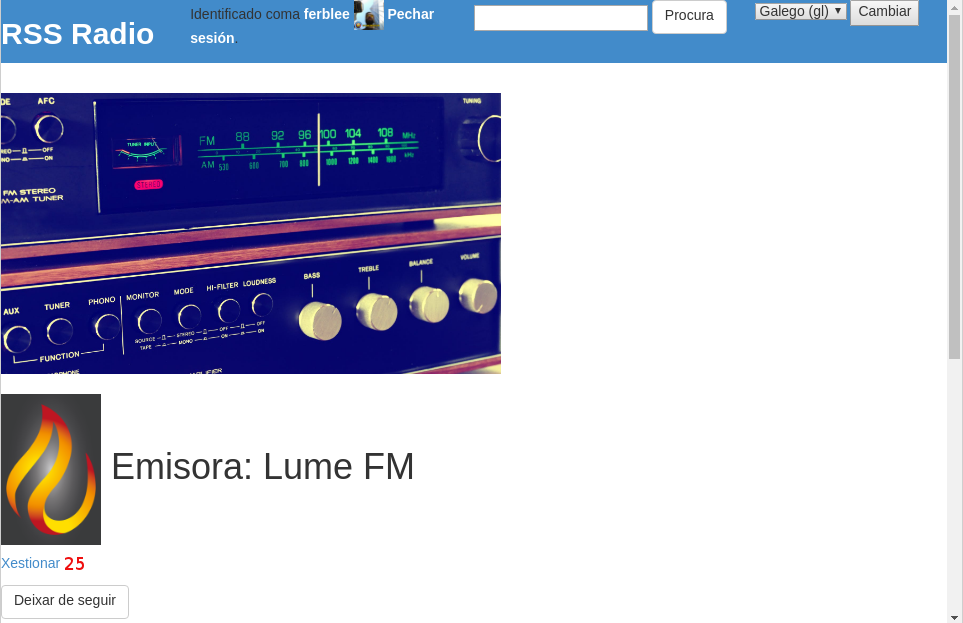
\includegraphics[scale=0.43,keepaspectratio=true]{./images/usermanual/um-stationd2.png}
	\caption{Vista de detalles de emisora: Nova emisora.}
	\label{fig:um-stationd2}
\end{figure}

\begin{figure}[H]
	\centering
	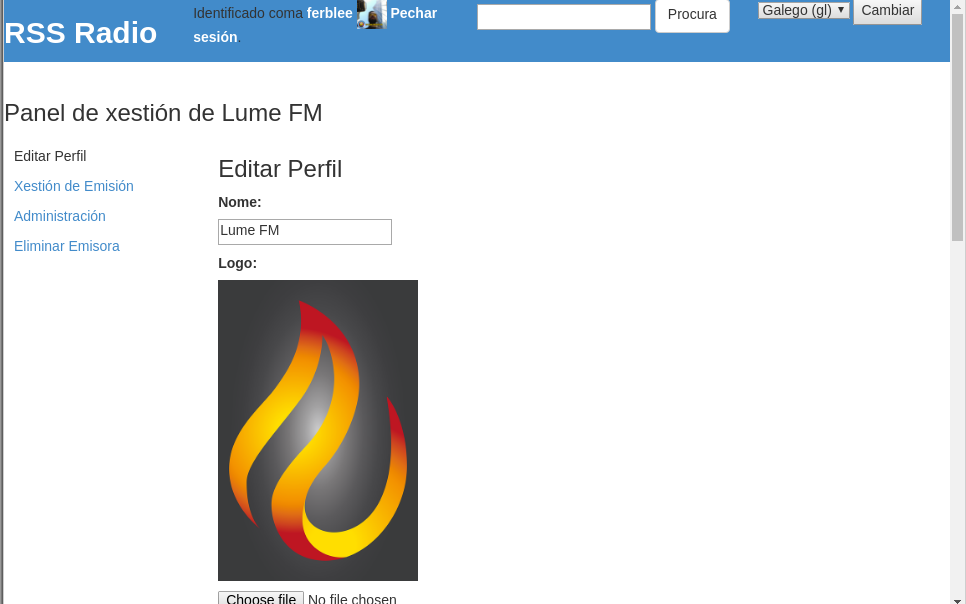
\includegraphics[scale=0.43,keepaspectratio=true]{./images/usermanual/um-edstation1.png}
	\caption{Panel de xestión de emisora: Editar perfil.}
	\label{fig:um-edstation1}
\end{figure}

\begin{figure}[H]
	\centering
	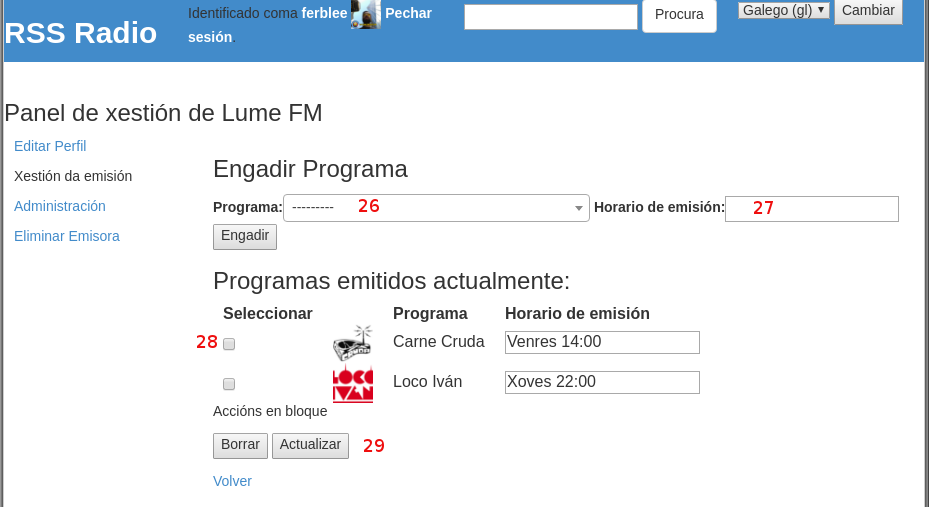
\includegraphics[scale=0.43,keepaspectratio=true]{./images/usermanual/um-edstation2.png}
	\caption{Panel de xestión de emisora: Xestionar emisión.}
	\label{fig:um-edstation2}
\end{figure}

\subsubsection{Xestionar administradores}
\label{xadmin}
Vista amosada na figura \ref{fig:um-edstation3}. Desde aí pódenselle conceder e revogar aos usuarios permisos sobre a emisora. Só os usuarios de nivel propietario poden acceder a esta vista. 

\textbf{Importante:} O propietario orixinal da emisora é o usuario que a crea. Este pode nomear outros propietarios pero, unha vez nomeados, non os poderá \say{degradar} xa que estarán ao seu mesmo nivel. Recoméndase prudencia á hora de conceder os permisos.

\begin{itemize}
	\item \textbf{30:} Selector de usuario. Úsase para seleccionar o usuario ao que se lle queiran dar permisos.
	\item \textbf{31:} Selector de permisos. Poden ser de administrador (limitados) ou de propietario (totais)
	\item \textbf{32:} Área de usuarios xa con permisos. Ás filas seleccionadas aplicaráselles á acción definida en \textbf{33}.
	\item \textbf{33:} Botóns de acción. Determinan se os usuarios seleccionados son para borrar ou para actualizar os seus permisos.
\end{itemize}


\subsubsection{Borrar emisora}

Vista amosada na figura \ref{fig:um-edstation4}. Desde aí pódese eliminar a emisora. So os propietarios teñen acceso a esta vista.

\begin{figure}[H]
	\centering
	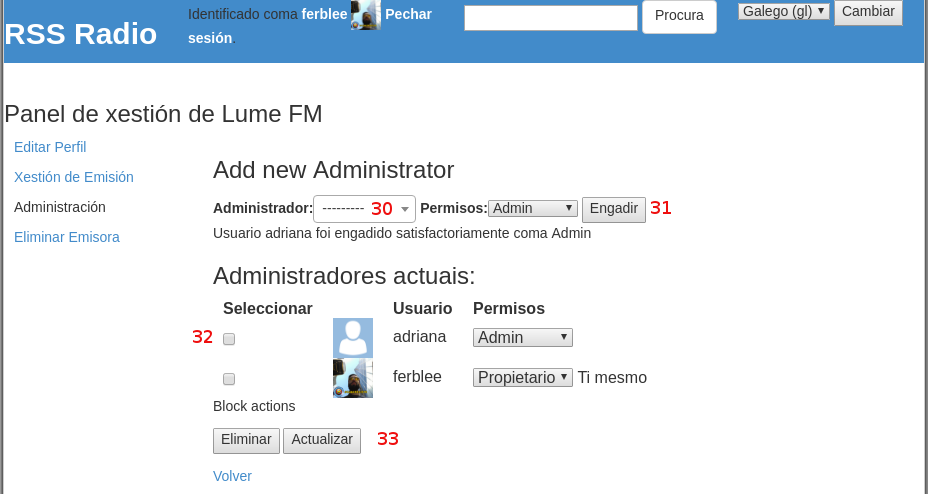
\includegraphics[scale=0.43,keepaspectratio=true]{./images/usermanual/um-edstation3.png}
	\caption{Panel de xestión de emisora: Xestionar administradores.}
	\label{fig:um-edstation3}
\end{figure}

\begin{figure}[H]
	\centering
	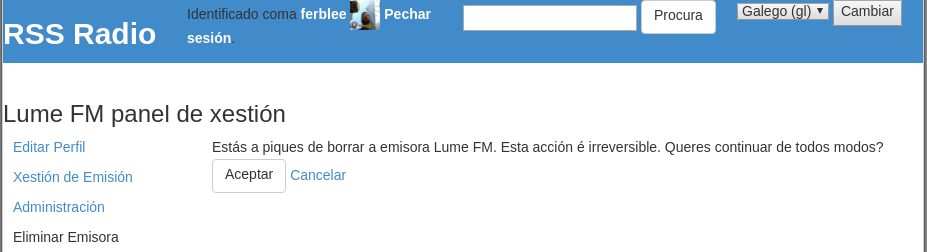
\includegraphics[scale=0.43,keepaspectratio=true]{./images/usermanual/um-edstation4.png}
	\caption{Panel de xestión de emisora: Borrar emisora.}
	\label{fig:um-edstation4}
\end{figure}


\subsection{Crear un programa}

Ao igual que a emisora, é necesario acceder ao menú de engadir contido a través do botón \textbf{5} na figura \ref{fig:um-index-anon} e cubrir o formulario que se ve na figura \ref{fig:um-add-program}.

Se os datos introducidos son correctos, rediríxese ao usuario á páxina de detalles da novo programa (figura \ref{fig:um-programd2}), onde tamén poderemos ver todos os seus episodios, creados automaticamente. O usuario creador do programa ten permisos de \say{propietario} sobre el e mailos seus episodios.

\begin{itemize}
	\item \textbf{34:} Opcións de compartición. As opcións son \textit{libre} e \textit{desactivada} segundo se desexe que as emisoras poidan emitir libremente o novo programa ou non.  
	\item \textbf{35:} Opcións de comentarios. As opcións son \textit{Permitir} e \textit{Deshabilitar} os comentarios nos episodios do novo programa.
\end{itemize}


\begin{figure}[H]
	\centering
	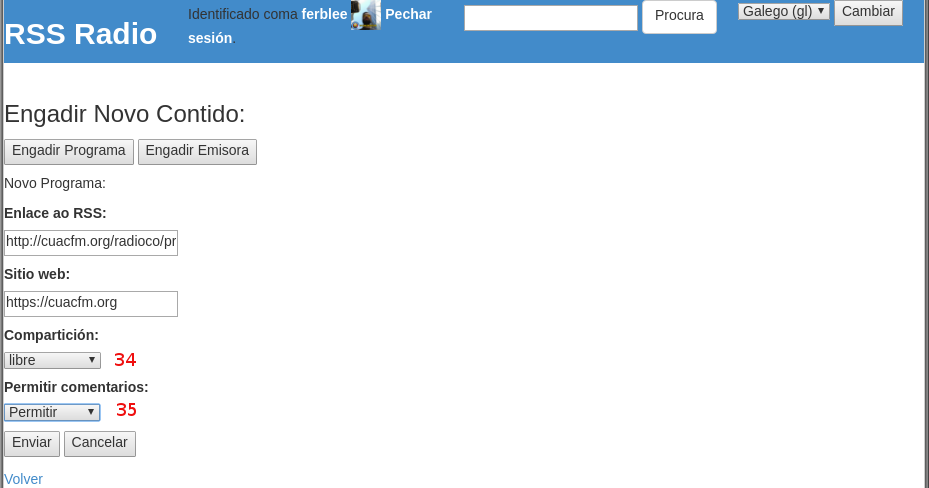
\includegraphics[scale=0.43,keepaspectratio=true]{./images/usermanual/um-add-program.png}
	\caption{Engadir programa.}
	\label{fig:um-add-program}
\end{figure}

\begin{figure}[H]
	\centering
	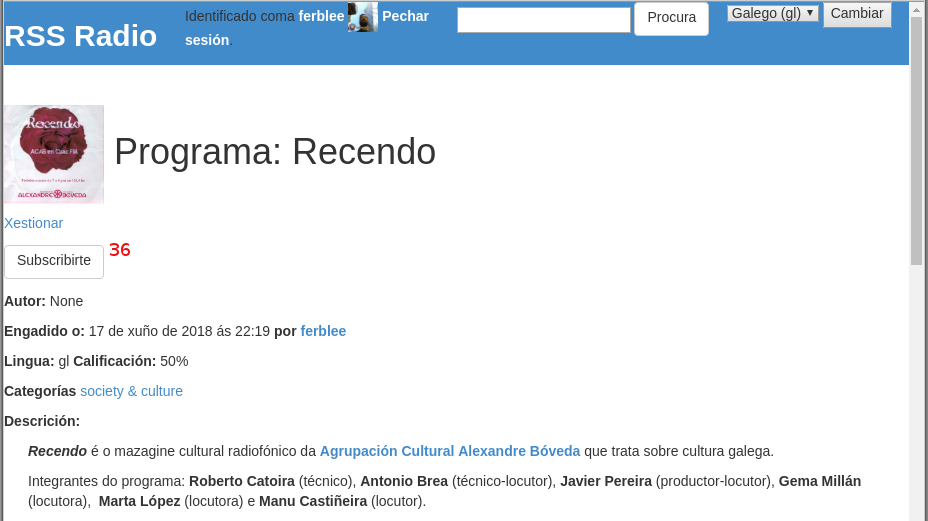
\includegraphics[scale=0.43,keepaspectratio=true]{./images/usermanual/um-programd2.png}
	\caption{Vista de detalles de program: Novo programa.}
	\label{fig:um-programd2}
\end{figure}


\subsection{Xestionar un programa}

Se o usuario é propietario ou xestor dun programa, poderá ver o botón marcado coma \textbf{36} na figura \ref{fig:um-programd2} que leva ao panel de xestión do programa. O sistema non ofrece ferramentas de xestión non edición dos episodios de xeito individual. As opcións definidas para o programa aplicaranse a todos os seus episodios sen excepcións.

As ferramentas que se utilizan neste panel funcionan do mesmo xeito que as do panel de xestión de emisora. Ante calquera dúbida, consultar as seccións \ref{xe} e \ref{xadmin}.

Neste panel pódense realizar as seguintes operacións:

\subsubsection{Editar perfil}

Esta vista é semellante á de editar o perfil da emisora, porén, podemos ver na \ref{fig:um-edprogram1} que as opcións son, aquí, moito máis limitadas debido a que a información é obtida dunha fonte externa (o ficheiro RSS) e non da entrada manual de datos por parte do usuario.

\begin{figure}[h]
	\centering
	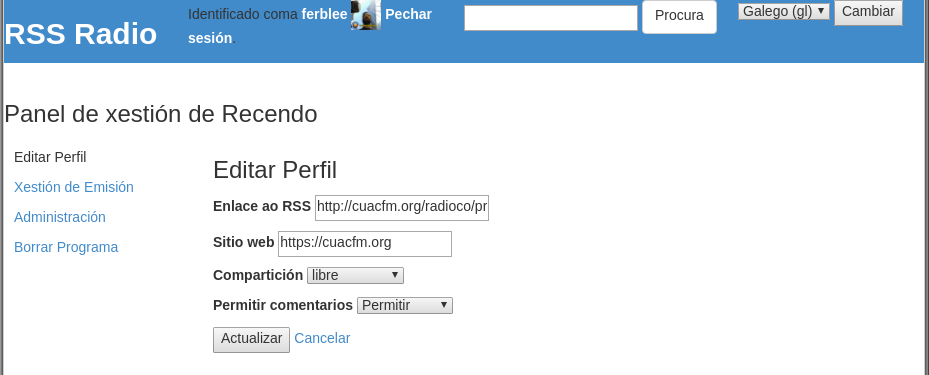
\includegraphics[scale=0.43,keepaspectratio=true]{./images/usermanual/um-edprogram1.png}
	\caption{Panel de xestión de programa: Editar perfil.}
	\label{fig:um-edprogram1}
\end{figure}

\subsubsection{Xestionar emisión}

Vista amosada na figura \ref{fig:um-edprogram2}. O sistema dá a oportunidade ao propietario do programa de cesar a emisión nunha emisora, pero, como é lóxico, non de modificar o seu horario de emisión nesa emisora. 

\begin{figure}[h]
	\centering
	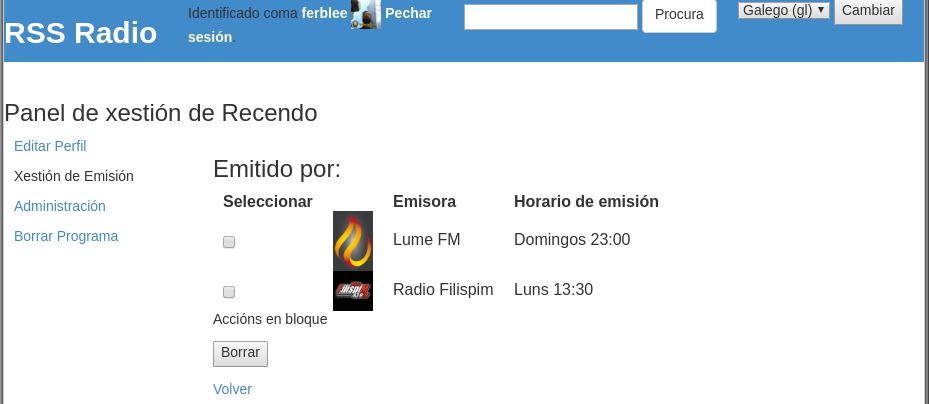
\includegraphics[scale=0.43,keepaspectratio=true]{./images/usermanual/um-edprogram2.png}
	\caption{Panel de xestión de programa: Xestionar emisión.}
	\label{fig:um-edprogram2}
\end{figure}

\subsubsection{Xestionar administradores}

Vista amosada na figura \ref{fig:um-edprogram3}. Desde aí pódenselle conceder e revogar aos usuarios permisos sobre a emisora. Só os usuarios de nivel propietario poden acceder a esta vista. 

\textbf{Importante:} O propietario orixinal do programa é o usuario que o crea. Este pode nomear outros propietarios pero, unha vez nomeados, non os poderá \say{degradar} xa que estarán ao seu mesmo nivel. Recoméndase prudencia á hora de conceder os permisos.

\begin{figure}[h]
	\centering
	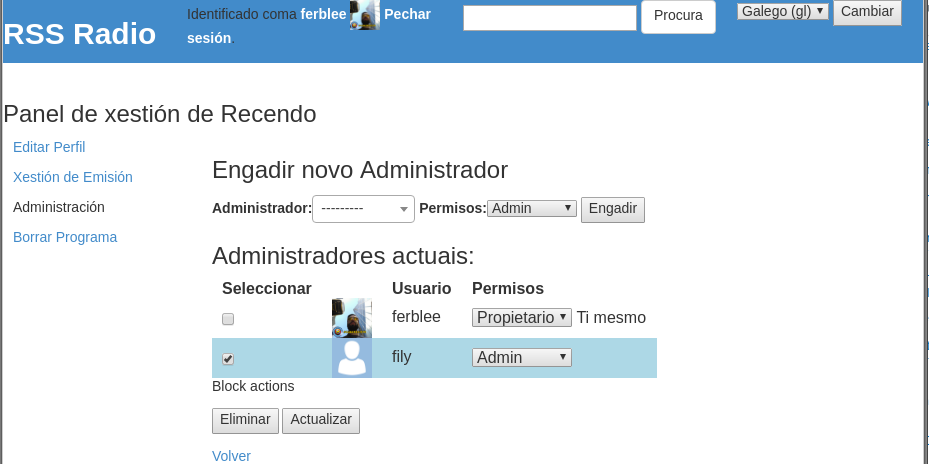
\includegraphics[scale=0.43,keepaspectratio=true]{./images/usermanual/um-edprogram3.png}
	\caption{Panel de xestión de programa: Xestionar administradores.}
	\label{fig:um-edprogram3}
\end{figure}


\subsubsection{Borrar programa}

Vista amosada na figura \ref{fig:um-edprogram4}. Desde aí pódese eliminar o programa. So os propietarios teñen acceso a esta vista.

\textbf{Importante:} O borrado dun programa implica a eliminación de todos os seus episodios así como das súas imaxes relacionadas. Os datos non serán recuperables.

\begin{figure}[h]
	\centering
	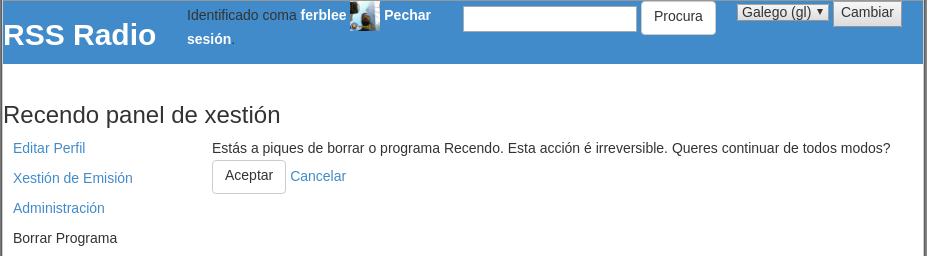
\includegraphics[scale=0.43,keepaspectratio=true]{./images/usermanual/um-edprogram4.png}
	\caption{Panel de xestión de programa: Borrar programa.}
	\label{fig:um-edprogram4}
\end{figure}